
\documentclass[12pt,a4paper]{article}

% Türkçe %
\usepackage[utf8]{inputenc} %Türkçe karakterler için
\usepackage[T1]{fontenc}
\renewcommand{\tablename}{Tablo}
\renewcommand{\figurename}{Şekil}
\renewcommand{\indexname}{Dizin}
\renewcommand{\listfigurename}{Şekiller}
\renewcommand{\listtablename}{Tablolar}
\renewcommand{\contentsname}{İçindekiler}
\renewcommand{\refname}{Kaynaklar}
% Türkçe %

\usepackage{pdfpages}
\usepackage{geometry}
\usepackage{graphicx} %Resim koymak için
\usepackage{times} %Times fontu
\usepackage{graphicx}
\usepackage[nottoc]{tocbibind}
\usepackage{url}

\begin{document}

    \pagenumbering{gobble}
    \begin{titlepage}
   \begin{center}
      \begin{large}
         \vspace*{0.5cm}
         GAZİ ÜNİVERSİTESİ \\
         MÜHENDİSLİK FAKÜLTESİ \\
         BİLGİSAYAR MÜHENDİSLİĞİ

         \vfill
         BM495  BİLGİSAYAR PROJESİ \\
         SPMP BELGESİ

         \vfill
         Abdullah Akalın\\Karim El Guermai\\Muhammed Emre Emrah\\

         \vfill
         \vspace{0.5cm}
         01.11.2017
      \end{large}
   \end{center}
\end{titlepage}

    \newpage

    \pagenumbering{roman}
    \tableofcontents
    \newpage

    \pagenumbering{arabic}

    \section{Derin Öğrenme: Tanımlar ve Yöntemler}
	Derin öğrenme, yapay öğrenme konusunun bir alt dalıdır. Adını, neredeyse tüm derin öğrenme
	algoritmalarının dayandığı yapay sinir ağlarındaki "saklı katman" denilen, girdi ve çıktı
	arasındaki verinin işlenip bir sonraki katmana geçtiği derin yapıdan alır. İnsan beynindeki
	nöronların çalışma prensibini taklit etmeye çalışır. En iyi avantajı, kendi kendine feature’lar
	oluşturup kullanabilmesidir. Dezavantajı ise, çok fazla veriye ihtiyaç duymasıdır.

    \begin{figure}[!h]
        \begin{center}
            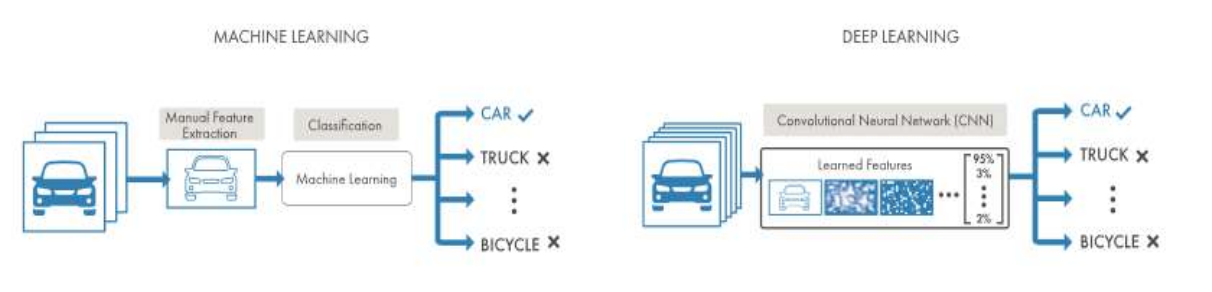
\includegraphics[width=\linewidth]{resimler/dl1.png}
            %\caption{Başarılı renklendirme örnekleri.\cite{colorful}}
            %\label{fig:color}
        \end{center}
    \end{figure}

	\subsection{Evrişimli Yapay Sinir Ağları (CNN)}
	Yaygın olarak görüntü işlemede sahne tanıma (scene recog.) ve obje konumlama, tanımada
	kullanılır. Bir resimdeki ana yapıları (vektörler, arklar vb.), küçük objelerin dahi küçük
	yapıtaşlarını öğrenir. Bunları kendi kendine bir feature haline getirebilir. Bu sayede daha
	büyük yapıları tanır. Şaşırtıcı derecede başarılı sonuçlar elde edilebilir.

	\subsection{Regresyon Yapay Sinir Ağları (RNN)}
	Yapay sinir ağlarının regresyon ile kullanılmasıdır.

	\subsection{Pekiştirmeli Öğrenme}
	Başka alanlarda da kullanılıyor olup, sistemin davranışı sırasında istenilen şeyleri yapınca ödül,
istenmeyen şeyleri yapınca ceza puanı almasını sağlayarak; ve puana etki eden inputlara ağırlık
verilerek, sonuçta sistemin istenmeyen davranışları yapmamasını sağlamak amaçlıdır.

    \section{Proje İncelemeleri}

    \subsection{Görüntü Renklendirme}
    \textbf{Çalışmanın özgün adı:} Colorful Image Colorization \cite{colorful}. \\
    \textbf{Yazarlar:} Richard Zhang, Phillip Isola, Alexei A. Efros \\
    \textbf{Kısa Özet:} Bu çalışmanın amacı gri tonlamalı bir fotoğrafın girdi olarak alınıp,
    çıktı olarak aynı fotoğrafın renklendirilmiş halini üretmektir (\figurename{} \ref{fig:color}). Çıkan görüntünün asıl
    görüntüyle aynı renklerde olması beklenmemektedir. Esas amaç insan gözü tarafından ayırt
    edilemeyecek uygunlukta görüntüler çıkartmaktır. \\
    \textbf{Kullanılan Yöntemler:} Çalışmada temel olarak CNN (Convolutional Neural Network)'ler ve "Self-Supervised Feature
    Learning" yöntemleri kullanılmıştır. \\
    \textbf{Veri Seti:} ImageNet\cite{imagenet}, SUN\cite{sun} görüntü verileri. \\
    \textbf{Sonuç:} Yapılan deneylerde insan gözlemcilerin \%32 oranında, üretilmiş renkli görüntüleri
    gerçek görüntüler zannettikleri tespit edilmiştir\footnote{Örnek görüntüler için: http://richzhang.github.io/colorization/}.

    \begin{figure}[!h]
        \begin{center}
            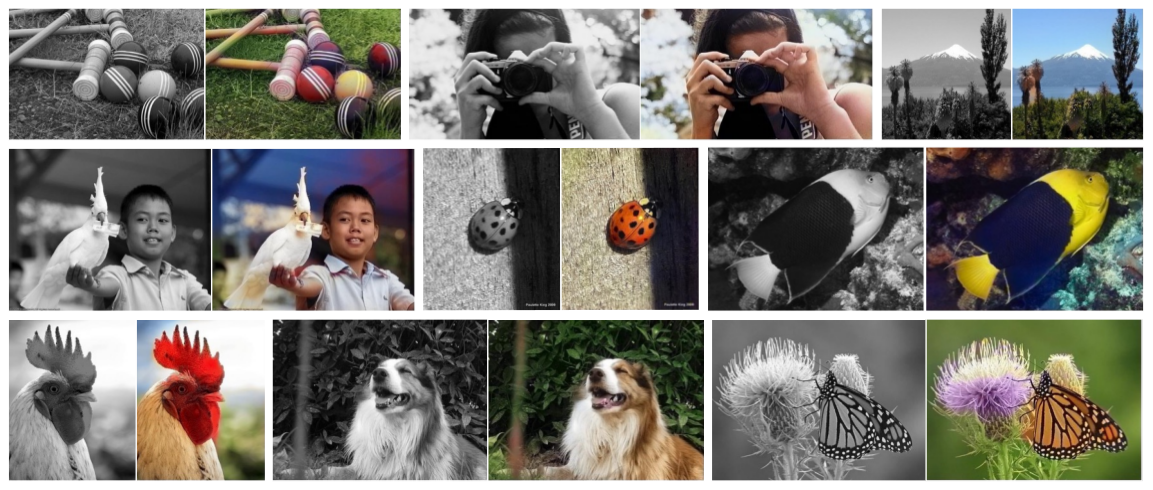
\includegraphics[width=\linewidth]{resimler/color.png}
            \caption{Başarılı renklendirme örnekleri.\cite{colorful}}
            \label{fig:color}
        \end{center}
    \end{figure}

    \subsection{Resimlerde Stil Transferi}
    \textbf{Çalışmanın özgün adı:} Semantic Style Transfer and Turning Two-Bit Doodles into Fine Artwork \cite{trans}. \\
    \textbf{Yazar:} Alex J. Champandard \\
    \textbf{Kısa Özet:} Bu çalışmanın amacı bir sanat eserindeki karakteristikleri derin öğrenme yöntemleriyle
    öğrenip, basit bir karalamayı bu sanat eserine benzer karakteristikte bir görüntüye dönüştürmektir (\figurename{} \ref{fig:style}).
    Amaç, gerçekleştirilmesi çok zor olan birebir taklit olmayıp, insan gözlemci tarafından, esas alınan esere
    karakteristik olarak benzeyen görüntü üretmektir.\\
    \textbf{Kullanılan Yöntemler:} Çalışmada temel olarak "VGG Convolutional Neural Networks"\cite{vgg} yöntemleri ve
    verileri kullanılmıştır. \\
    \textbf{Sonuç:} Birebir örtüşme aranmadığı sürece kabul edilebilir sonuçlar gözlemlenmiştir\footnote{Örnek görüntüler için: https://github.com/alexjc/neural-doodle}.

    \begin{figure}
        \begin{center}
            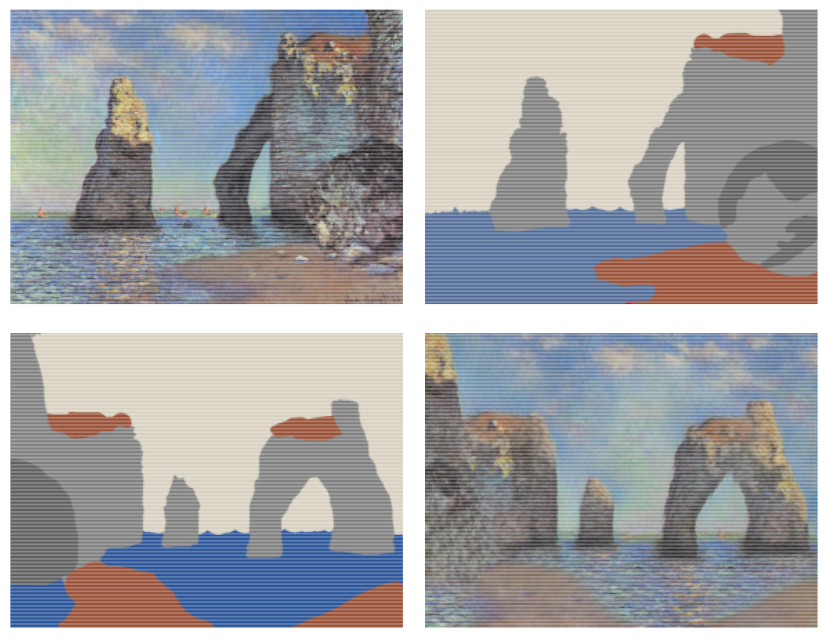
\includegraphics[width=300px]{resimler/style.png}
            \caption{Artistik transfer örneği. Asıl görüntü sol-üstte, bilgisayar tarafından çıkartılan taslak sağ-üstte,
            insan tarafından çizilen taslak sol-altta, bilgisayar tarafından oluşturulan çıktı sağ-altta bulunmaktadır.\cite{trans}}
            \label{fig:style}
        \end{center}
    \end{figure}

    \subsection{El Yazısıyla Yazılmış Rakamları Tanıma}
    \textbf{Çalışmanın özgün adı:} Handwritten Digits Recognition \cite{minst}. \\
    \textbf{Yazarlar:} 
	Yann LeCun, Courant Institute (NYU), Corinna Cortes (Google Labs, New York), Christopher J.C. Burges (Microsoft Research, Redmond) \\
    \textbf{Kısa Özet:} Çalışmanın amacı, girdi olarak verilen el yazısı ile yazılmış rakamın hangi
rakam olduğunu tanımaktır \cite{minst}. \\
    \textbf{Kullanılan Yöntemler:} Deep learning yöntemleri dahil olmak üzere bir çok yöntem ve
algoritma kullanılmıştır. \\
	\textbf{Veri Seti:} MNIST SD-1 ve SD-3 veri setleri kullanılmıştır. Toplam 60,000 training
images, 60,000 training labels; 10,000 test images ve 10,000 test labels kullanılmıştır. Test
setlerinin yarısı güzel yazı yazan kişiler, diğer yarısı da anlaşılması daha zor yazan kişiler
tarafından alınmıştır.\\

    \subsection{Google Street View Apartman Numaraları}
    \textbf{Çalışmanın özgün adı:} The Street View House Numbers (SVHN) Dataset \cite{svhn}. \\
    \textbf{Yazarlar:} 
	Yuval Netzer, Tao Wang, Adam Coates, Alessandro Bissacco, Bo Wu,
Andrew Y. \\
    \textbf{Kısa Özet:} Apartman tabelalarında yer alan (genelde mavi renkli) apartman numaralarını tanıma ve üzerinde yazan numarayı elde etme. \\
	\textbf{Veri Seti:} Training için 73257 rakam, test için ise 26032 rakam bulunuyor. Ek olarak
ise, okunması biraz daha kolay olan 531131 rakam bulunmaktadır.
Veriler iki formattadır. Birincisinde, orijinal çekilen fotoğraflar, ikincisinde ise 32x32 olacak
şekilde, sayıların ortalandığı görüntüler şeklindedir. \\

    \subsection{Drivers, Focusing on Your Driving!}
    \textbf{Author:} Yundong Zhang \cite{drvr}\\
    \textbf{Summary:} The aim of this project is to build a computer vision system that detects the distracted behaviors of
drivers and alarms them when they perform one. The distracted behaviors can be texting, drinking,
talking on the phone and etc. \\
    \textbf{Methods:} Two methods were used to classify drivers behaviors based on the input images: Support Vectors
Machines (SVM) and phone and Convolutional neural network (CNN). \\
	\textbf{Data Set:} The data is available on Kaggle Dataset, It is named: Stated Farm Distracted Driver. It consists of 10
classes of image data taken in a car for training purposes. It has22424 training images and 79727 test
images each of size 640x280 pixels. \\
    \textbf{Result:} Please refer to Şekil \ref{fig:vgg}.

    \begin{figure}
        \begin{center}
            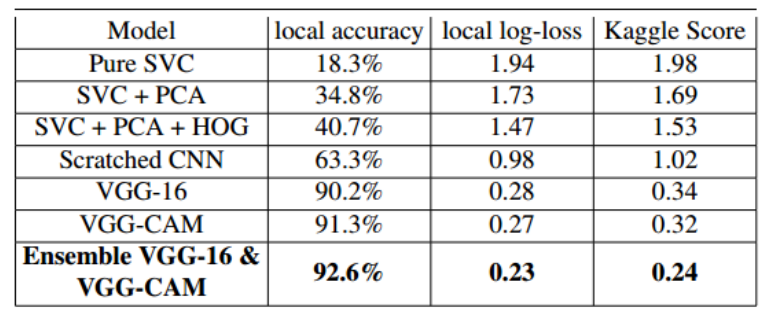
\includegraphics[width=300px]{resimler/vgg.png}
            \caption{Model score.}
            \label{fig:vgg}
        \end{center}
    \end{figure}

    \subsection{Stack Overflow Query Outcome Prediction}
    \textbf{Author:} Robbie M. Jones, David Lin  \cite{sower}\\
    \textbf{Summary:} The project basically builds a classifier that predicts whether a user’s question will be closed along with
the reason for closure. This will reduce the work of moderators and will gives better insights for users to
ask valid questions. \\
    \textbf{Methods:} In this project, the models were trained using logistic regression, Support Vector Machines (SVMs) and
boosting. \\
	\textbf{Data Set:} The data used for this project was found on StackExchange Data Explorer and then was preprocessed.
Preprocessing included separating closed and non-closed questions, restricting time-sensitive attributes
and applying various transformations to textual data. \\
    \textbf{Result:} The most accurate models were the linear SVM followed by the radical SVM. The classifiers did a good
job separating non-closed questions from closed questions, but not as good when it comes to
differentiate between the different reasons for closure (Şekil \ref{fig:fig}).

    \begin{figure}
        \begin{center}
            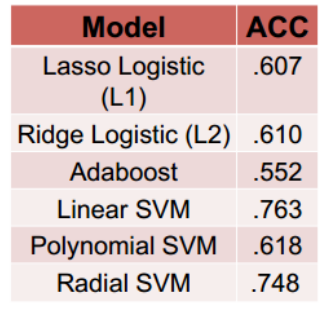
\includegraphics[width=150px]{resimler/fig.png}
            \caption{Classification summary.}
            \label{fig:fig}
        \end{center}
    \end{figure}

    \newpage
    \bibliography{kaynakca/kaynakca}
    \bibliographystyle{ieeetr}

\end{document}


